\documentclass[a4paper,11pt]{jsarticle}


% 数式
\usepackage{amsmath,amsfonts,amssymb}
\usepackage{bm}
% 画像
\usepackage[dvipdfmx]{graphicx}
\usepackage[dvipdfmx]{color}
\usepackage{siunitx}
\usepackage{wrapfig}
\usepackage{cases}
\usepackage{dcolumn}
\makeatletter
\newcommand{\figcaption}[1]{\def\@captype{figure}\caption{#1}}
\newcommand{\tblcaption}[1]{\def\@captype{table}\caption{#1}}
\makeatother

\usepackage{listings,jvlisting}
\lstset{
basicstyle={\ttfamily},
identifierstyle={\small},
commentstyle={\smallitshape},
keywordstyle={\small\bfseries},
ndkeywordstyle={\small},
stringstyle={\small\ttfamily},
frame={tb},
breaklines=true,
columns=[l]{fullflexible},
numbers=left,
xrightmargin=0zw,
xleftmargin=3zw,
numberstyle={\scriptsize},
stepnumber=1,
numbersep=1zw,
lineskip=-0.5ex
}

\begin{document}

\title{vGyへの貢献をどう評価するか}
\author{Hiro Hirabayashi}
\date{\today}
\maketitle

現状考えている評価方法は
\begin{enumerate}
  \item 力積
  \item 仕事量
  \item $\int\sigma (vy_G)ay_G dt$ で表される単位付き力積
\end{enumerate}

\section{Case: 単純なばね(落下なし)}

\begin{figure}[h]
  \centering
  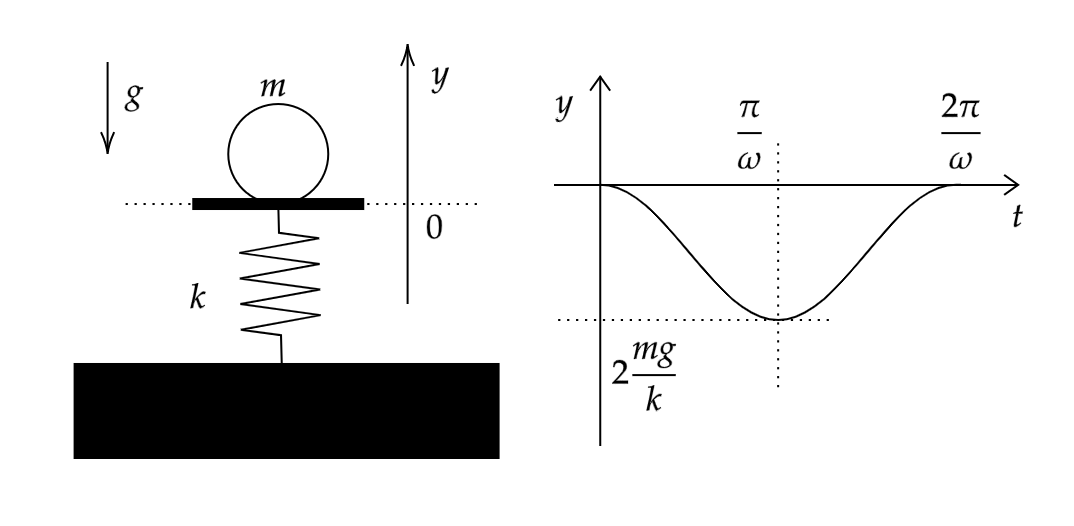
\includegraphics[width = 0.6\textwidth]{simple_string.png}
  \caption{}
  \label{simple_string.png}
\end{figure}

\subsection{準備}
\begin{align}
  ma &= -mg - ky
  \\ &= -k\left(y + \frac{mg}{k}\right)
\end{align}
\begin{align}
  \therefore 
  \left(y+\frac{mg}{k}\right) = A\sin(\omega t) + B\cos(\omega t)
\end{align}
ただし、$t=0$で$y=0,\dot{y}=0$より、
\begin{align}
  y &= -\frac{mg}{k} + \frac{mg}{k}\cos(\omega t)
  \\ &= \frac{mg}{k}\left(-1+\cos(\omega t)\right)
\end{align}

そんで、ばね板から離れる条件はもちろん
\begin{align}
  F_y = 0 \Leftrightarrow ky = 0
\end{align}
*ばね板にちゃんと質量(M)を持たせると、
\begin{align}
  \begin{cases}
    M\ddot{y} &= -F_y - ky
    \\ m\ddot{y} &= F_y
  \end{cases}
\end{align}
\begin{align}
  \therefore (M + m)\ddot{y} = - ky
\end{align}
になって質量が変わるだけ。だけどシミュレーションするときには板に質量をもたせておいたほうが安心かな。

離ばねまでちょうど1周期だから
$\frac{2\pi}{\omega}$
だけかかる。

\subsection{貢献}
先に結論だけ書く。
保存力だけだとうまく判断できない。
\begin{enumerate}
  \item 力積
  重力による力積は
  \begin{align}
    \int_0^{\frac{2\pi}{\omega}} -mg dt = -mg \frac{2\pi}{\omega}
  \end{align}

  ばねの弾性による力積は
  \begin{align}
    \int_0^{\frac{2\pi}{\omega}} -ky dt &= -k \int_0^{\frac{2\pi}{\omega}} \frac{mg}{k}\left(-1+\cos(\omega t)\right)
    \\ &= -mg \int_0^{\frac{2\pi}{\omega}} \left(-1+\cos(\omega t)\right) dt
    \\ &= -mg \left[-t+\frac{1}{\omega}\sin(\omega t)\right]_0^{\frac{2\pi}{\omega}}
    \\ &= -mg \left( -\frac{2\pi}{\omega} \right) = mg \frac{2\pi}{\omega}
  \end{align}

  離ばね地点において元の状態に戻っているから、正味の力積が0になるのは妥当。

  \item 仕事量
  重力による仕事量は
  \begin{align}
    \int_0^{\frac{2\pi}{\omega}} -mg\cdot\dot{y} dt = \int_{t=0}^{t=\frac{2\pi}{\omega}} -mg dy = 0
  \end{align}
  位置エネルギーの変化分だから0になるのは妥当。

  ばねの弾性による仕事量も
  \begin{align}
    \int_0^{\frac{2\pi}{\omega}} -ky \cdot\dot{y} dt
    &= \int_{t=0}^{t=\frac{2\pi}{\omega}} -kydy
    \\&= \left[-\frac{1}{2}ky^2\right]_{t=0}^{t=\frac{2\pi}{\omega}} = 0
  \end{align}
  位置エネルギーの変化分だから0になるのは妥当。

  離ばね地点において元の状態に戻っているから、正味の仕事量が0になるのは妥当。

  \item $\int\sigma (vy_G)ay_G dt$ で表される単位付き力積
  重力による単位付き力積は
  \begin{align}
    \int_0^{\frac{\pi}{\omega}} -mg\cdot(-1) dt + \int_{\frac{\pi}{\omega}}^{\frac{2\pi}{\omega}} -mg\cdot(1) dt
    &= mg\frac{\pi}{\omega} + \left(-mg\frac{\pi}{\omega}\right) = 0
  \end{align}

  ばねの弾性による単位付き力積は
  \begin{align}
    \int_0^{\frac{\pi}{\omega}} -ky\cdot(-1) dt 
    &+ \int_{\frac{\pi}{\omega}}^{\frac{2\pi}{\omega}} -ky\cdot(1) dt
    \\ &= k \int_0^{\frac{\pi}{\omega}} \frac{mg}{k}\left(-1+\cos(\omega t)\right)
    - k \int_{\frac{\pi}{\omega}}^{\frac{2\pi}{\omega}} \frac{mg}{k}\left(-1+\cos(\omega t)\right)
    \\&= mg \left[-t+\frac{1}{\omega}\sin(\omega t)\right]_0^{\frac{\pi}{\omega}}
    - mg \left[-t+\frac{1}{\omega}\sin(\omega t)\right]_{\frac{\pi}{\omega}}^{\frac{2\pi}{\omega}}
    \\&= mg \left( -\frac{\pi}{\omega} + 0 \right)
    - mg\left( -\frac{\pi}{\omega} + 0 \right)
    \\ &= 0
  \end{align}

\end{enumerate}


\end{document}